\def\argmin{\mathop{\text{\rm arg\,min}}}
\mathchardef\mh="2D
\def\ACDC{AC\kern.01ex\Lightning\kern.01ex DC}

\msection{Estimation and Inference Under Shape Restrictions (Aim 3) }
\label{sec:aim3}
\vskip-10pt \background{} Shape restrictions such as monotonicity,
convexity, and concavity provide a natural way of limiting the
complexity of many statistical estimation problems.  Shape-constrained
estimation is not as well understood as more traditional nonparametric
estimation involving smoothness constraints.  For instance, the
minimax rate of convergence for multivariate convex regression has yet
to be rigorously established in full generality, although covering and
bracketing number bounds have been recently established
\citep{kim2014global}.  Even the one-dimensional case is challenging,
and has been of recent interest \citep{guntusen:13}.

Estimation of convex functions arises naturally in several
applications.  Examples include geometric programming \citep{Boyd04},
computed tomography \citep{Prince:90}, target reconstruction
\citep{Lele:92}, image analysis \citep{Golden:06} and circuit design
\citep{Hannah:12}.  Other applications include queuing theory
\citep{Chen:01} and economics, where it is of interest to estimate
concave utility functions \citep{Pratt:68}.  
Beyond cases where the assumption of convexity is
natural, the convexity assumption can be attractive as a
tractable, nonparametric relaxation of the linear model.  

The convex regression problem is naturally
formulated using finite dimensional convex optimization, with no
tuning parameters for smoothness.  
We have recently begun to study the problem of variable selection in
high dimensional multivariate convex regression.  Assuming that the regression function
is convex and sparse, our goal is to identify the relevant variables.
We have shown that it suffices to estimate a sum of one-dimensional convex
functions---an additive model---leading to significant computational and statistical
advantages \citep{xu:14}.  This is in contrast to general nonparametric regression,
where fitting an additive model can result in false negatives.

To briefly explain, the infinite-dimensional nonparametric convex regression
$ \min_{\mbox{\scriptsize $f$ convex}} \sum_i (y_i - f(x_i))^2$
is equivalent to the finite dimensional quadratic program
$\min_{f,\beta} \sum_i (y_i - f_i)^2$ subject to the
subgradient constraints $f_j \geq f_i + \beta_i^T (x_j - x_i) $.
This optimization is subject to the statistical curse of dimensionality.
To carry out scalable variable selection, we
have devised a two-stage quadratic programming procedure.  In
the first stage, we fit a convex additive model, imposing a sparsity
penalty.  In the second stage, we fit a concave function on the
residual for each variable.  This non-intuitive second
stage is in general necessary.   We call this the \ACDC{} algorithm:
\def\C{{\mathcal C}}

\begin{enumerate}
\item \textit{AC Stage}: Estimate an additive convex model
\begin{equation*}
\{\hat{f}_k\}, \hat \mu  = \argmin_{f_1,...,f_p \in
  \C^1, \,\mu\in\reals} 
   \frac{1}{n} \sum_{i=1}^n \Big(y_i - \mu - \sum_{k=1}^p f_k(x_{ik}) \Big)^2 
       + \lambda \sum_{k=1}^p \| f_k \|_\infty.
\end{equation*}
\item \textit{DC Stage}: If $\| \hat{f}_k \|_\infty = 0$, estimate a
  decoupled concave function
\begin{equation*}
\hat{g}_k = \argmin_{g_k \in \mh{}\C^1} 
   \frac{1}{n} \sum_{i=1}^n \Big( y_i - \hat \mu - \sum_{k'} \hat{f}_{k'}(x_{ik'}) 
    - g_k(x_{ik})\Big)^2 
      + \lambda \| g_k \|_\infty.
\end{equation*}
\item Estimated support $\hat S_n = \{ k \,:\, \| \hat{f}_k \|_\infty > 0 
  \textrm{ or } \| \hat{g}_k \|_\infty > 0 \}$.
\end{enumerate}

\begin{figure}[t]
\begin{center}
%\ \vskip-20pt
\begin{tabular}{ll}
\hskip-10pt
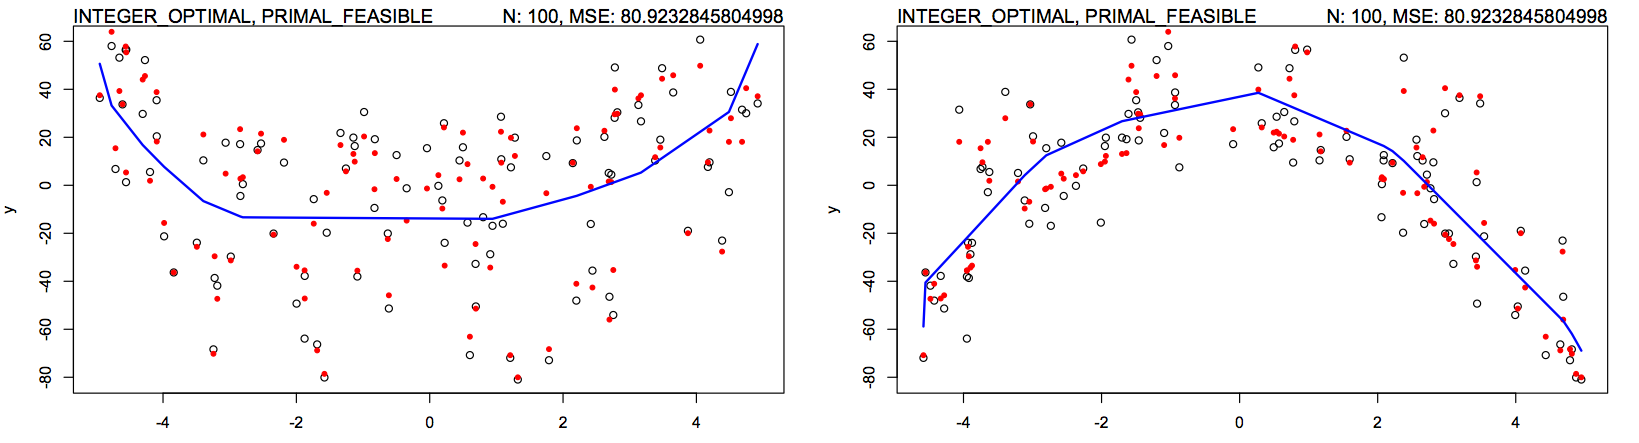
\includegraphics[width=.59\textwidth]{figs/cp-sim} \quad & 
\quad \begin{minipage}[b]{2.3in}
\small\linespread{1.0}\selectfont
\stepcounter{figure}
\vskip-10pt
Figure \arabic{figure}. Simple illustration
of convexity pattern estimation.  We estimate
a two-dimensional additive model, where each component
is either convex or concave; there are $2^p$ possible
convexity patterns.  
%This illustates the solution
%using a mixed integer SOCP optimization.  This can
%also be approached using a convex optimization
%which a nonstandard verison of the lasso.
\vskip2pt{\ }
\end{minipage}
\\[-10pt]
\end{tabular}
\end{center}
\end{figure}

We have proven that this 
procedure is faithful in the population setting, meaning that it
results in no false negatives, under mild assumptions on the density
of the covariates.  Our second result is a finite sample statistical
analysis of the procedure, where we upper bound the statistical rate
of convergence.  Specifically, ``sparsistent'' variable selection is
achievable with sample complexity $n$ satisfying
$ n^{4/5} \geq C s^5 \sigma^2 \log^2 p$
where $s$ is the number of true relevant variables \citep{xu:14}.  
The proof of this
result exploits recent bounds on bracketing numbers for
convex function classes due to \cite{kim2014global}.


\project{Convexity pattern estimation}
Suppose we have an additive model with a sum of 
convex and concave functions.
Then estimation is a quadratic program, with no smoothing parameters.
But what if we don't know the {\it\bfseries convexity pattern}---which
  functions are convex and which are concave?  Can it be learned?
Solving this problem will lead to a new, powerful approach
to nonparametric modeling.

More specifically, the model is
\begin{gather*}
Y = \sum_{j=1}^p z_j\, f_j(x_j)  + \varepsilon \\
z_j\in \{-1, 1\}, \quad f_j\ \text{convex}
\end{gather*}
and our objective is to decode
$z = (z_1,\ldots, z_p) \in \{-1, 1\}^p$ from observed data
$\{(X_i, Y_i)\}_{i=1}^n$, $X_i\in\reals^p$, $Y_i\in\reals$.
One approach is to formulate a mixed integer second-order cone program,
minimizing the squared error for an additive model $\sum_j (f_j(x_j) +
g_j(x_j))$
where $f_j$ is convex and $g_j$ is concave.  We then impose
second order cone constraints $\|f_j\| \leq z_jB$ and 
$\|g_j\| \leq w_jB$ with the constraint $z_j + w_j \leq 1$.  When
we impose the integer constraints $z_j, w_j \in \{0,1\}$, this
results in a mixed integer SOCP.    
We have experimented with this using the R package \texttt{Rmosek} to
call the Mosek mixed integer SOCP code.  The procedure works well; however,
the run time will in general be exponential, and
the lack of a duality theory for such optimization makes analysis difficult.

A better, convex approach is the following.  Consider the optimization
\begin{align*}
\min_{f,g,\beta,\gamma,z,w}\quad & \sum_{i=1}^n \Bigl(Y_i - \sum_{j=1}^p (f_{ij}+g_{ij})\Bigr)^2 \\
\text{subject to}\quad 
  & \text{convexity constraints on $f_{j}$} \\
  & \text{concavity constraints on $g_{j}$} \\
  & \sum_{j=1}^p \left\{\beta_{(n)j} - \beta_{(1)j} + \gamma_{(1)j} -
  \gamma_{(n)j}\right\} \leq L
\end{align*}
where $\beta_{(1)j}, \beta_{(n)j}, \gamma_{(1)j}, \gamma_{(n)j}$ are
the first and last subgradient vectors of $f_j$ and $g_j$.
This can be thought of as a nonstandard type of lasso.  
This works very well in simulation.  However, the analysis
will require new advances beyond the standard primal-dual witness
approach. We will fully develop the theory and algorithms for this approach.



\project{Estimation of SOS-convex densities} Log-concavity is often an
appropriate shape constraint for density estimation.  A density $f(x)$
is said to be log-concave if $f(x) = \exp(-s(x))$ where $s(x)$ is a
convex function.  \cite{Cule:10} have studied nonparametric
log-concave density estimation.  They show that with probability one
there exists a unique optimal solution $\hat f_n$ of the nonparametric
log-likelihood $\ell(f) = \sum_{i=1}^n \log f(X_i)$ and that $\log\hat
f_n$ is a piecewise affine ``tent function'' on the convex hull $C_n$
of the data.  Thus, $\hat f_n$ is not in general smooth.  Computing
$\hat f_n$ is formulated as a non-smooth convex optimization problem
with is solved through Shor's $r$-algorithm. Unfortunately, this does not scale to
dimensions much larger than five with current technology.

We will study a different approach, restricting our attention
to the class of log-SOS-concave functions $f(x) = \exp(-s(x))$ where
$s(x)$ is an SOS-convex polynomial 
\citep{lasserre:09}.  While checking a polynomial's convexity is
in general strongly NP-hard, as shown by \cite{ahmadi:13},
an algebraic sum of squares (SOS) is a sufficient condition 
for convexity that can be certified by solving a semidefinite program.
We propose to exploit this construction to develop algorithms
based on projected stochastic gradient descent, where
an SDP is solved in each gradient step to project onto 
the cone of SOS-concave functions.  This requires
MCMC to estimate expectations.  
Since our algorithm is an iterative procedure
employing stochastic gradient descent, we will
leverage recent results on sequential sampling for log-concave
densities \citep{Narayanan:13}.



%\project{Detection of shape-constrained signals}

\project{Utility function estimation}
One natural application of convex regression is modeling
utility functions in economics and marketing.
Many human behaviors can be modeled as a consumer selecting one item
from among a set of alternatives.  Examples include buying a product
on Amazon, choosing the bus or car for
commuting~\citep{ortuzar1994modelling}, deciding where to buy a
house~\citep{nechyba1998community}, and even choosing where to commit
a crime~\citep{bernasco2009offenders}. The discrete choice model (DCM)
originated in econometrics~\citep{mcfadden1973conditional} as a
general method to model such finite choice problems. The DCM measures
the attractiveness of item $i$ to consumer $n$ by a utility function
$f(\mathbf{x}_i, \mathbf{s}_n)$ where $\mathbf{x}_i, \mathbf{s}_n$ are
feature vectors of the item and the consumer, respectively. The
consumer is more likely to pick item $i$ over the alternatives if the
utility $f(\mathbf{x}_i, \mathbf{s}_n)$ is higher. The AI and machine
learning communities have in recent years rediscovered the DCM as a
form of \emph{preference learning} \citep{furnkranz2010preference,
  chu2005preference}.

Our work on variable selection in shape-constrained regression can be
applied to the DCM.  This is pertinent since people tend to make
decisions based on a few important cues or
factors~\citep{shah2008heuristics}. Good variable selection methods
can give insight into how consumers make choices.  While estimation of
a low dimensional concave utility function for the DCM is studied by
Matzkin using parametric distributional assumptions
\citep{matzkin1991semiparametric}, we are unaware of previous results
on variable selection in the DCM in the high dimensional nonparametric
context.   We will also study how a \textit{mixture} of
utility functions can be estimated, specializing the model
to groups of consumers.  For this goal, we
will investigate nonparametric versions
of the method of moments 
for mixtures \citep{icml_liang,anima_colt}.  We are interacting
with faculty and students in Chicago's Booth School of Business
on initial research on these topics.


%\project{Shape-constrained mixtures}

% method of moments

